% Chapter Template

\chapter{Preliminary Models} % Main chapter title

\label{Chapter:Classification} % Change X to a consecutive number; for referencing this chapter elsewhere, use \ref{ChapterX}

In this chapter we present the models that where designed in the early stage of the thesis. The aim of this work was to understand better the problem, ie. explore different input sizes, types of models, data augmentation techniques and hyper-parameters and explore the possibilities of using deep learning for successfully solving this task. They where published in \citep{jdelatorre2016}.

\section{Introduction}

In the last decade, several attempts to automatize the DR diagnosis through images of the eye fundus have been tested. They are basically focused on applying well-known pattern recognition models. In this work, we want to apply a Deep Convolutional Neural Network (DCNN) model, as it has been proven to be a very effective algorithm to solve general image classification problems. DCNN is a supervised learning model for automatic classification that does not require any pretreatment of the images, nor any feature analysis. 

Deep learning techniques are focused on learning multiple levels of representation and abstraction that help to make sense of the hidden information in data such as images. In this way having a complete set of correctly classified images and without having any a priori understanding of the features required to make the classification, the system is able to learn the properties of the image that minimize a defined cost function that is direct or indirectly related with the classification score index that has to be optimized.
In this chapter we show that a DCNN is able to learn from data the most important features to make the classification of retinal images into the five DR categories, without the need of a hand-crafted feature extraction process.

In this chapter we explore methods for classifying retina images into the five different classes of DR defined in chapter \ref{Chapter:Background}, that are:

\begin{enumerate}
	\item [0.]\setcounter{enumi}{0} - No apparent retinopathy
	\item - Mild Non-Proliferative Diabetic Retinopathy (NPDR)
	\item - Moderate NPDR
	\item - Severe NPDR
	\item - Proliferative DR
\end{enumerate}

The chapter is organized as follows: we present the related work, next we explain the characteristics of the available data and why deep learning techniques can be applied over them, next we explain the methodology used for solving the problem, we show the obtained results and finally we expose the conclusions and further steps for improving the results.

\section{Related work}

Traditional models of pattern recognition in images since the late 50s have been based on extracting hand-crafted fixed engineered features or fixed kernels from the image and, then, using a trainable classifier on top of those features to get the final classification. Using this model, the problem of the DR detection has been tackled by feature extraction using on hand models targeted to the detection of microaneurisms, haemorrhages and exudates in retinal images (e.g. \citep{sudha2014}, \citep{torrents15}, etc). 

This type of approach requires a good understanding of disease mechanisms to be able to find the important features present in the image. This knowledge is specific of the problem to be solved, requires a lot of labor time and is task specific and thereby not reusable for other different classification problems.

Deep learning is a new powerful method for supervised learning. By adding more layers and more units within a layer of a neural network, we can represent functions of increasing complexity. Training must be done on sufficiently large annotated image data sets. In computer vision classification problems, neural networks have largely displaced the traditional approaches based on handcrafted features. They have proved to be the best available method for solving the biggest classification challenges, like for example IMAGENET \citep{ILSVRC15}. In this previous type of image analysis problems, distinct objects should be recognized on different types of images. In the case of DR classification, all images are very similar (as they are retina photos) and very small and vague lesions have to be detected at different locations in order to find the correct severity category of DR. This chapter, thus, wants to study the performance of DCNNs for this kind of medical image analysis.

\section{Data}

We use the EyePACS dataset presented in chapter \ref{Chapter:Background}. We split the dataset using random selection in two disjoint sets. The training set contains 35,126 images; 25,810 of class 0, 2,443 of class 1, 5,292 of class 2, 873 of class 3 and 708 of class 4. The test set contains a total of 53,576 images; 39,533 of class 0, 3,762 of class 1, 7,861 of class 2, 1,214 of class 3 and 1,206 of class 4.


\section{Methodology for retinal image classification}

All the state-of-the-art architectures for supervised deep learning over images (e.g. AlexNet \citep{Krizhevsky:2012}, GoogleNet \citep{googlenet} and VGGNet \citep{vggnet}) are based on convolutional neural networks (CNNs). A set of convolutional layers with dimensional down-sizing blocks between them, also known as pooling layers, extract the statistical information from the data (feature extraction) that is passed to the posterior layers to construct more elaborate abstractions (features of features) that are useful for the classification. As a final stage a fully connected set of layers perform the classification based on the information coming from the last layers of the convolutional network. This kind of structure provides an end to end learning process, where either the classes or the features are learned from data with no human intervention.

Next we explain the different phases of the DCNN construction for performing DR detection based on the available data: evaluation function, data pre-processing and data augmentation, model, training, testing and probabilistic combination of the models of both eyes.

\subsection{Evaluation function}

The performance of the classification model is measured using the quadratic weighted kappa  (QWK) index  (see eq. \ref{ccia2016:eq:kappa}), defined previously in chapter \ref{Chapter:Background}. As a brief summary, QWK, also known as Cohen's Kappa, measures inter-rater agreement for categorical items in multi-class classification problems \citep{kappa}, penalizing the discrepancy quadratically with the distance from the correct class. It is generally thought to be a more robust measure than simple percent agreement calculation, since QWK takes into account the agreement occurring by chance. This metric typically varies from 0 (random agreement) to 1 (complete agreement). Negative values are also possible, the maximum possible negative value (-1) indicates a complete disagreement between classes.
Being $O_{i,j}$ the observed values, $E_{i,j}$ the expected ones and $C$ number of classes, QWK is defined as:

\begin{equation}\label{ccia2016:eq:kappa}
\kappa = 1 - \frac{ \sum_{i=1}^C \sum_{j=1}^C \omega_{i,j} O_{i,j} }
{\sum_{i=1}^C \sum_{j=1}^C  \omega_{i,j} E_{i,j}}
\quad \textrm{where} \quad \omega_{i,j} = \frac{(i-j)^2}{(C - 1)^2}
\end{equation}

%\caption{Quadratic Weighted Kappa expression, 


The QWK coefficient is used to compare the performance of different prediction models and with the performance of the human experts \citep{kappa-benchmark}. Individual human experts report values of QWK of about 0.80 in the prediction of the correct class in the DR disease. This value is considered excellent because small discrepancies between the class prediction does not affect the treatment of the disease. The most important is the differentiation between presence or absence of the disease. 

\subsection{Data pre-processing and data augmentation}

%The original images have diverse original resolutions and, thus, they need to be resized to a common value. After this step a data augmentation and a posterior normalization is done.

Firstly, DCNNs require large data-sets in order to avoid overfitting. A class balanced data-set is also desirable as well \citep{class-imbalance}. One of the proven approaches that has good results to get more data from small data-sets is to use data augmentation techniques \citep{Krizhevsky:2012}. The data augmentation is done in two stages: first a copy of the training examples of the small classes is done until they have the same number of images as the biggest class. This generates an equilibrated training set. After this first step, to every image the next transformations are applied in order to diversify the training examples:

\begin{itemize}
	%\item Resizing, $\pm1$\% random uniform
	\item Cropping, random uniform
	\item Rotation (\ang{0} to \ang{360}), random uniform
	\item Mirroring ( X and Y axes), random uniform
	\item Brightness correction, random gaussian ($\sigma$ = 0.1)
	\item Contrast correction, random gaussian ($\sigma$ = 0.1)
\end{itemize}

All these transformations are applied to every image of the balanced training set and redone for every training epoch. This transformations assure that every image of the training set is different between each other for every epoch, making the final prediction invariant to rotation, brightness and contrast over the training set.

Secondly, DCNNs perform better when then input data is normalized by having mean equal to 0 and standard deviation equal to 1, on each channel (RGB). Thus, a normalization must be done on each image.

\subsection {Model}

The well-known LeCun et al. architecture has been taken \citep{LeCun:98}. It is composed by a series of convolutional layers followed by activation function blocks, with some max-pooling dimensional reducing blocks. At the end, a final fully connected layer performs the classification and, finally, a softmax output layer gives a probability estimation of every class  (Figure \ref{fig:traditional-convolutional-network}). 


\begin{figure}[h]
	\centering
	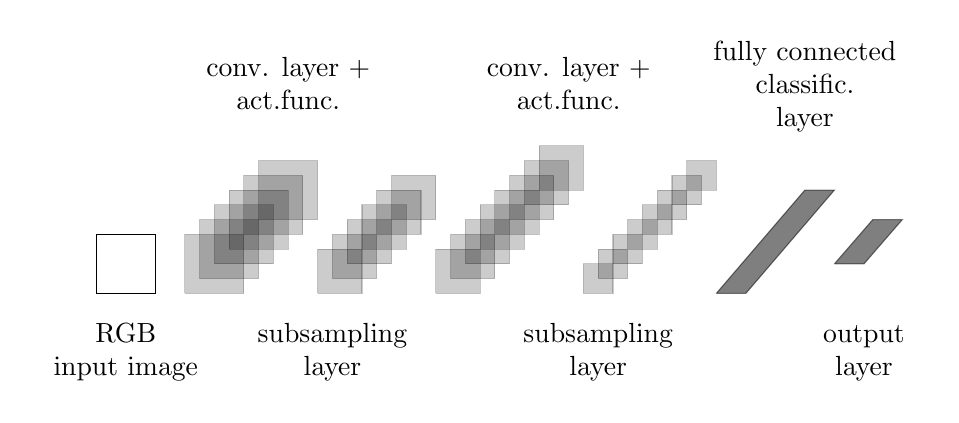
\begin{tikzpicture}[scale=0.75]
	\node at (0.5,-1){\begin{tabular}{c}RGB\\ input image\end{tabular}};
	
	\draw (0,0) -- (1,0) -- (1,1) -- (0,1) -- (0,0);
	
	\node at (3.25,3.5){\begin{tabular}{c}conv. layer + \\ act.func.\end{tabular}};
	
	\draw[fill=black,opacity=0.2,draw=black] (2.75,1.25) -- (3.75,1.25) -- (3.75,2.25) -- (2.75,2.25) -- (2.75,1.25);
	\draw[fill=black,opacity=0.2,draw=black] (2.5,1) -- (3.5,1) -- (3.5,2) -- (2.5,2) -- (2.5,1);
	\draw[fill=black,opacity=0.2,draw=black] (2.25,0.75) -- (3.25,0.75) -- (3.25,1.75) -- (2.25,1.75) -- (2.25,0.75);
	\draw[fill=black,opacity=0.2,draw=black] (2,0.5) -- (3,0.5) -- (3,1.5) -- (2,1.5) -- (2,0.5);
	\draw[fill=black,opacity=0.2,draw=black] (1.75,0.25) -- (2.75,0.25) -- (2.75,1.25) -- (1.75,1.25) -- (1.75,0.25);
	\draw[fill=black,opacity=0.2,draw=black] (1.5,0) -- (2.5,0) -- (2.5,1) -- (1.5,1) -- (1.5,0);
	
	\node at (4,-1){\begin{tabular}{c}subsampling\\ layer\end{tabular}};
	
	\draw[fill=black,opacity=0.2,draw=black] (5,1.25) -- (5.75,1.25) -- (5.75,2) -- (5,2) -- (5,1.25);
	\draw[fill=black,opacity=0.2,draw=black] (4.75,1) -- (5.5,1) -- (5.5,1.75) -- (4.75,1.75) -- (4.75,1);
	\draw[fill=black,opacity=0.2,draw=black] (4.5,0.75) -- (5.25,0.75) -- (5.25,1.5) -- (4.5,1.5) -- (4.5,0.75);
	\draw[fill=black,opacity=0.2,draw=black] (4.25,0.5) -- (5,0.5) -- (5,1.25) -- (4.25,1.25) -- (4.25,0.5);
	\draw[fill=black,opacity=0.2,draw=black] (4,0.25) -- (4.75,0.25) -- (4.75,1) -- (4,1) -- (4,0.25);
	\draw[fill=black,opacity=0.2,draw=black] (3.75,0) -- (4.5,0) -- (4.5,0.75) -- (3.75,0.75) -- (3.75,0);
	
	\node at (8,3.5){\begin{tabular}{c}conv. layer +\\ act.func.\end{tabular}};
	
	\draw[fill=black,opacity=0.2,draw=black] (7.5,1.75) -- (8.25,1.75) -- (8.25,2.5) -- (7.5,2.5) -- (7.5,1.75);
	\draw[fill=black,opacity=0.2,draw=black] (7.25,1.5) -- (8,1.5) -- (8,2.25) -- (7.25,2.25) -- (7.25,1.5);
	\draw[fill=black,opacity=0.2,draw=black] (7,1.25) -- (7.75,1.25) -- (7.75,2) -- (7,2) -- (7,1.25);
	\draw[fill=black,opacity=0.2,draw=black] (6.75,1) -- (7.5,1) -- (7.5,1.75) -- (6.75,1.75) -- (6.75,1);
	\draw[fill=black,opacity=0.2,draw=black] (6.5,0.75) -- (7.25,0.75) -- (7.25,1.5) -- (6.5,1.5) -- (6.5,0.75);
	\draw[fill=black,opacity=0.2,draw=black] (6.25,0.5) -- (7,0.5) -- (7,1.25) -- (6.25,1.25) -- (6.25,0.5);
	\draw[fill=black,opacity=0.2,draw=black] (6,0.25) -- (6.75,0.25) -- (6.75,1) -- (6,1) -- (6,0.25);
	\draw[fill=black,opacity=0.2,draw=black] (5.75,0) -- (6.5,0) -- (6.5,0.75) -- (5.75,0.75) -- (5.75,0);
	
	\node at (8.5,-1){\begin{tabular}{c}subsampling\\ layer\end{tabular}};
	
	\draw[fill=black,opacity=0.2,draw=black] (10,1.75) -- (10.5,1.75) -- (10.5,2.25) -- (10,2.25) -- (10,1.75);
	\draw[fill=black,opacity=0.2,draw=black] (9.75,1.5) -- (10.25,1.5) -- (10.25,2) -- (9.75,2) -- (9.75,1.5);
	\draw[fill=black,opacity=0.2,draw=black] (9.5,1.25) -- (10,1.25) -- (10,1.75) -- (9.5,1.75) -- (9.5,1.25);
	\draw[fill=black,opacity=0.2,draw=black] (9.25,1) -- (9.75,1) -- (9.75,1.5) -- (9.25,1.5) -- (9.25,1);
	\draw[fill=black,opacity=0.2,draw=black] (9,0.75) -- (9.5,0.75) -- (9.5,1.25) -- (9,1.25) -- (9,0.75);
	\draw[fill=black,opacity=0.2,draw=black] (8.75,0.5) -- (9.25,0.5) -- (9.25,1) -- (8.75,1) -- (8.75,0.5);
	\draw[fill=black,opacity=0.2,draw=black] (8.5,0.25) -- (9,0.25) -- (9,0.75) -- (8.5,0.75) -- (8.5,0.25);
	\draw[fill=black,opacity=0.2,draw=black] (8.25,0) -- (8.75,0) -- (8.75,0.5) -- (8.25,0.5) -- (8.25,0);
	
	\node at (12,3.5){\begin{tabular}{c}fully connected \\classific.\\layer\end{tabular}};
	
	\draw[fill=black,draw=black,opacity=0.5] (10.5,0) -- (11,0) -- (12.5,1.75) -- (12,1.75) -- (10.5,0);
	
	\node at (13,-1){\begin{tabular}{c}output\\ layer\end{tabular}};
	
	\draw[fill=black,draw=black,opacity=0.5] (12.5,0.5) -- (13,0.5) -- (13.65,1.25) -- (13.15,1.25) -- (12.5,0.5);
	\end{tikzpicture}
	\caption[Architecture of a 4 layer CNN]{Architecture of a 4 layer CNN: two convolutional layers, one fully connected classification layer and the final output layer}
	\label{fig:traditional-convolutional-network}
\end{figure}

Some of the parameters of this model are the following: input size, number of layers, number of filters per convolution layer, size of the convolution, number and size of classification layers, activation function, optimization and regularization methods to be used. Due to the high number of parameters involved, these systems have a lot of versatility and there is not a unique solution to a problem. Different configurations can perform well solving the same problem.

\subsection{Training procedure}

As a multi-class classification problem, a log-loss function is used to perform the optimization in the learning stage. The original training set is splitted in two random subsets: one with 90\% of the data and other with 10\%. The last one is used as a cross validation set for hyperparameter selection.  QWK results are calculated every epoch either for the training or the test set. The model chosen is the one that maximizes the QWK over the cross validation set. In all models a ReLU or leaky ReLU \citep{Dahl2013} activation function is used. In all layers a batch normalization \citep{batch-norm} is applied before the activation function in order to reduce the gradient vanishing problem that occurs in deep networks, reduce the internal covariance shift and improve the regularization. As an additional regularizer a dropout \citep{baldi2013} (p=0.5) is performed before the final classification layer. L2 regularization has been tested with no significative improvements in the final classification results. A random initialization based in the Kaiming\&He approach \citep{kaiming} is used for all the networks. When deep networks are randomly initialized using fixed standard deviations (e.g., 0.01), very deep models (e.g., >8 conv layers) have difficulties to converge, as reported by the VGG team \citep{DBLP:journals/corr/SimonyanZ14a}. Kaiming method takes into account the particularities of rectifier non-linearities. Initializing the weights of every layer randomly with 0 mean and $\sqrt{2/n_l}$ standard deviation ( being $n_l$ the number of connections of layer l) we get a desired zero-mean Gaussian distribution in the weight distribution. Biases are initialized to zero. All models are optimized using stochastic gradient descent with Nesterov momentum.

\subsection{Testing procedure}

The network is trained with a data augmented scheme that include rotations. Presumably an ensemble \citep{ensembling} that includes rotated versions of the original image would perform better that the single original image. Using a trained network with a significant accuracy, different ensemble schemes are tested over the cross validation set to identify the one that maximizes the classification accuracy. 

\begin{table}[h!]
	\centering
	\scalebox{0.8}{
	\begin{tabular}{c c c c} 
		\hline
		Testing scheme & Predictions & $\kappa_{CV}$ \\ [0.5ex] 
		\hline\hline
		Baseline: Original image (crop center) & 1  & 0.669 \\
		Original + rot \ang{180} (crop center) & 2  & 0.683 \\
		Center, Left top, Left bottom, Right top, Right bottom cropped & 5 & 0.684 \\ 
		Original + Hflip + Vflip + rot \ang{180} & 4 & 0.686 \\
		Five \ang{72} rotated (crop center) & 5 & 0.699 \\
		All & 14 & 0.701 \\
		\hline
	\end{tabular}
	}
	\caption{Testing scheme performance results}
	\label{table-test-schemes}
\end{table}


\begin{figure}[h!]
	\centering
	\begin{subfigure}[t]{0.49\textwidth}
		\centering
		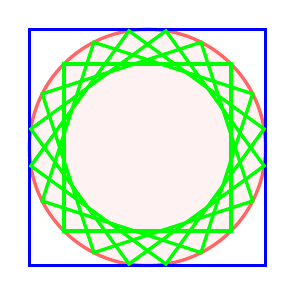
\begin{tikzpicture}[]
		\filldraw[color=red!60, fill=red!5, very thick](0,0) circle (1.5);
		\draw[blue, very thick] (-1.5,-1.5) rectangle (1.5,1.5);
		\draw[green, very thick, rotate around={0:(0,0)}](-1.06,-1.06) rectangle (1.06,1.06);
		\draw[green, very thick, rotate around={72:(0,0)}](-1.06,-1.06) rectangle (1.06,1.06);
		\draw[green, very thick, rotate around={144:(0,0)}](-1.06,-1.06) rectangle (1.06,1.06);
		\draw[green, very thick, rotate around={216:(0,0)}](-1.06,-1.06) rectangle (1.06,1.06);
		\draw[green, very thick, rotate around={288:(0,0)}](-1.06,-1.06) rectangle (1.06,1.06);
		\end{tikzpicture}
		\caption{Ensemble of five crops}
	\end{subfigure}%
	~ 
	\begin{subfigure}[t]{0.49\textwidth}
		\centering
		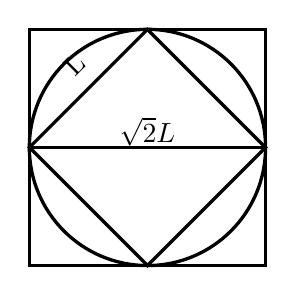
\begin{tikzpicture}[]
		\draw[black, very thick] (-1.5,-1.5) rectangle (1.5,1.5);
		\draw[black, very thick] (0, 0) circle (1.5);
		\draw[black, very thick, rotate around={45:(0,0)}](-1.06,-1.06) rectangle (1.06,1.06);
		\draw[black, very thick] (1.5,0.0) -- (-1.5,0.0);
		\draw (0.0,0.2) node {$\sqrt{2} L$};
		\node[label={[label distance=0.2,text depth=-1ex,rotate=45]L}] at (-0.75,0.75) {};
		\end{tikzpicture}
		\caption{Cropped vs image size}
	\end{subfigure}
	\caption{Testing ensemble used for evaluation}
	\label{fig:test-area}
\end{figure}

Table \ref{table-test-schemes} shows the accuracy of different testing schemes for a given model. The ensemble that performs the best is the one formed by all the 14 different evaluations. The Five \ang{72} scheme is only 0.002 points under the best tested scheme and reduces significantly the computation time required. Geometric means perform slightly better (average of 0.005 points of $\kappa$) than arithmetic means. The testing scheme chosen is the Five \ang{72} with geometric means due to its good compromise between computation costs and performance. In figure \ref{fig:test-area} we show a representation of the scheme. Blue square represents the image size, red circle the retinal image area and the five green squares, the areas of the image that are feeded to the neural network at test time. As the diagram show, most of the useful information for the classification is considered by one of the 5 different inputs.

\subsection{Probabilistic combination of the models of both eyes}

DR usually affects both eyes, specially when the illness is in high severity stages. We analyze the frequency of co-ocurrence of the five DR categories in the images of our dataset. The dataset is big enough to infer from the frequencies of co-occurrence of the classes, the conditional probabilities of having one class in one eye given another class in the other. 

In table \ref{class:tab:frequencies} we show the frequencies of occurrence of all the possible combinations of classes in both eyes. Notice that the larger frequencies are found in the diagonal, indicating that is usual that both eyes have similar levels of severity.

\begin{table}[ht!]
	\centering
	\begin{tabular}{c c c c c c c} 
		\hline
		Eyes & C0 & C1 & C2 & C3 & C4 & Sum\\ [0.5ex] 
		\hline\hline
		C0 & 12155 & 407 & 295 & 3 & 11 & 12871\\
		C1 & 435 & 600 & 171 & 2 & 4 & 1212\\
		C2 & 336 & 222 & 1998 & 96 & 50 & 2702\\
		C3 & 3 & 1 & 87 & 307 & 27 & 425\\
		C4 & 10 & 1 & 39 & 40 & 263 & 353\\		
		Sum & 12939 & 1231 & 2590 & 448 & 355 & 17563\\
		\hline
	\end{tabular}
	\caption[Frequencies of combined occurrence of classes in both eyes]{Frequencies of combined occurrence of classes in both eyes (left: rows, right: columns)}
	\label{class:tab:frequencies}
\end{table}

Using the frequentist interpretation of probability that defines an event's probability as the limit of its relative frequency in a large number of trials, we use this frequencies as an estimation for the calculation of the conditional probability. In table \ref{class:tab:probabilities} we show the values of all the calculated conditional probabilities of $P(Left|Right)$. The same can be done for the matrix $P(Right|Left)$.

\begin{table}[ht!]
	\centering
	\begin{tabular}{c c c c c c} 
		\hline
		Eyes & C0 & C1 & C2 & C3 & C4\\ [0.5ex] 
		\hline\hline
		C0 & 0.93940 & 0.33062 & 0.11389 & 0.00669 & 0.03098\\
		C1 & 0.03361 & 0.48740 & 0.06602 & 0.00446 & 0.01126\\
		C2 & 0.02596 & 0.18034 & 0.77142 & 0.21428 & 0.14084\\
		C3 & 0.00023 & 0.00081 & 0.03359 & 0.68526 & 0.07605\\
		C4 & 0.00077 & 0.00081 & 0.01505 & 0.08928 & 0.74084\\
		\hline
	\end{tabular}
	\caption[Conditional probabilities of occurrence of DR]{Probability of occurrence of Left eye class (rows) given the occurrence of the Right eye class (columns)}
	\label{class:tab:probabilities}
\end{table}

Using the Bayes rule, we can estimate the probability distribution of eye A, using the probability distribution of eye B given by our model. Being $P(Left)$ and $P(Right)$, the probability distributions obtained by our predictive model with the left image and the right image, respectively, we can estimate $P_L$ and $P_R$ using Eq. \ref{Bayes}. To merge the information obtained from out model $P(X)$ with the estimated coming from the other eye we calculate the arithmetic mean. The class with maximum value is the one selected for each eye.

\begin{equation}
\begin{aligned}
P_L = P(Left|Right)P(Right) \\ P_R = P(Right|Left)P(Left)\\
\end{aligned}
\label{Bayes}
\end{equation}

\section{Experiments}

Different experiments have been conducted to analyze the quality of the classification with different parameters of the DCNN. First, we perform an study of the best image size. Due to the type of image classification that is done, it is crucial to choose the right size of the input images in order to detect the important features involved in the RD severity detection. As explained before, cropping is part of the data augmentation scheme. The original size is chosen from the NN input size as $\sqrt{2}$ times the input size. In this way, due to the circular nature of the retina, we maximize the useful information of the square cropped from the center of the image (see Fig. \ref{fig:test-area}). The input sizes tested are:

\begin{itemize}
	\item Resizing to 181x181 cropped to 128x128 NN input
	\item Resizing to 362x362 cropped to 256x256 NN input
	\item Resizing to 543x543 cropped to 384x384 NN input
	\item Resizing to 724x724 cropped to 512x512 NN input
\end{itemize}

Different number of layers have also been studied for each image size.
In table \ref{table-results} are presented the higher classification rates obtained from the best models obtained for different input sizes. The number of layers of the best models are also shown.

\begin{table}[ht!]
	\centering
	\begin{tabular}{c c c c c} 
		\hline
		Layers & Input size & $\kappa_{test}$ & FN & FP \\ [0.5ex] 
		\hline\hline
		12 & (3,128,128) & 0.488 & 11.6\% & 11.5\% \\ 
		14 & (3,256,256) & 0.636 & 4.4\% & 28.7\% \\ 
		16 & (3,384,384) & 0.668 & 7.9\%& 14.9\%\\ 
		16 & (3,512,512) & 0.725 & 5.0\% & 11.9\% \\ 
		\hline
	\end{tabular}
	\caption{Best classification results for different input sizes}
	\label{table-results}
\end{table}

As the input size and the complexity of the network is increased the results obtained become better. Greater sizes give more definition of the underlying features in the image and the increased complexity of the network, increasing the number of layers, allows the construction of abstractions in the form of features of features that improves the classification accuracy. In table \ref{table:best-nn} we show the architecture details of the best model, a very deep network of 16 layers. This indicates that the distinction of the severity categories of DR in images in not an easy classification problem. With the 512x512 model we achieve a $\kappa_{test} = 0.725$ using only the information contained in the examined retine image.

Next, we study if the inclusion of the co-ocurrence information of both eyes is able to improve the quality of the classifier. Table \ref{table-results2} shows the final accuracy obtained combining both eyes for all the sizes. In the 512x512 model the accuracy is increased in about $0.03$ $\kappa$ points, a value that makes our model perform near human level expertise with a final $\kappa_{test} = 0.752$.

\begin{table}[ht!]
	\centering
	\begin{tabular}{c c c c c} 
		\hline
		Layers & Input size & $\kappa_{test}$ & FN & FP \\ [0.5ex] 
		\hline\hline
		12 & (3,128,128) & 0.555 & 11.2\%& 12.9\%\\ 
		14 & (3,256,256) & 0.661 & 4.4\% & 28.7\% \\ 
		16 & (3,384,384) & 0.722 & 11.2\% & 4.0\%  \\ 
		16 & (3,512,512) & 0.752 & 6.5\% & 7.0\% \\ 
		\hline
	\end{tabular}
	\caption{Best classification results adding the probabilistic information of both eyes}
	\label{table-results2}
\end{table}

\begin{table}[ht!]
	\centering
	\scalebox{0.9}{
	\begin{tabular}{c c c c} 
		\hline
		Layer & Type & Characteristics & Output Size \\ [0.5ex] 
		\hline\hline
		& Input & 3 RGB channels & (3,512,512) \\ 
		1 & Convolution & 8 filters 3x3 1,1 stride, 1,1 padding & (8,512,512) \\
		2 & Convolution & 16 filters 3x3 1,1 stride, 1,1 padding & (16,512,512) \\
		3 & Convolution & 16 filters 3x3 1,1 stride, 1,1 padding & (16,512,512) \\
		- & Max pooling & 2,2 size, 2,2 stride & (16,256,256) \\
		4 & Convolution & 32 filters 3x3 1,1 stride, 1,1 padding & (32,256,256) \\
		5 & Convolution & 32 filters 3x3 1,1 stride, 1,1 padding & (32,256,256) \\
		- & Max pooling & 2,2 size, 2,2 stride & (32,128,128) \\
		6 & Convolution & 64 filters 3x3 1,1 stride, 1,1 padding & (64,128,128) \\
		7 & Convolution & 64 filters 3x3 1,1 stride, 1,1 padding & (64,128,128) \\
		- & Max pooling & 2,2 size, 2,2 stride & (64,64,64) \\
		8 & Convolution & 128 filters 3x3 1,1 stride, 1,1 padding & (128,64,64) \\
		9 & Convolution & 128 filters 3x3 1,1 stride, 1,1 padding & (128,64,64) \\
		- & Max pooling & 2,2 size, 2,2 stride & (128,32,32) \\
		10 & Convolution & 128 filters 3x3 1,1 stride, 1,1 padding & (128,32,32) \\
		11 & Convolution & 128 filters 3x3 1,1 stride, 1,1 padding & (128,32,32) \\
		- & Max pooling & 2,2 size, 2,2 stride & (128,16,16) \\
		12 & Convolution & 128 filters 3x3 1,1 stride, 1,1 padding & (128,16,16) \\
		13 & Convolution & 128 filters 3x3 1,1 stride, 1,1 padding & (128,16,16) \\
		- & Max pooling & 2,2 size, 2,2 stride & (128,8,8) \\
		14 & Convolution & 256 filters 3x3 1,1 stride, 1,1 padding & (256,8,8) \\
		15 & Fully connected & 256 elements & (256) \\ [1ex] 
		16 & Softmax & 256 to 5 elements & 5 \\ [1ex] 
		\hline
	\end{tabular}
	}
	\caption{Best performing DCNN architecture}
	\label{table:best-nn}
\end{table}

\section{Conclusions}

In this chapter is shown that deep learning techniques are not only very effective for solving general classification tasks, but also for prediction in medical imaging. For our case study of diabetic retinopathy disease grading, having enough data our method is able to perform near human level expertise.

Work of next chapters will be centered on testing the newer schemes, the use of alternative cost functions that encode the prior information of the ordering of the classes and other more elaborated methods for combining the information coming from both eyes.
